\subsection{Configuration Replication Protocol}
\label{proto_config}

\dcamp configuration and topology state are replicated across the system using key-value pairs, with the keys laid out
in a hierarchical fashion. This lends itself nicely to PUB/SUB topic filtering.

For example, because a Metric node only needs the configuration values for its particular group, the node subscribes
only to the \texttt{"/CONFIG/<group-name>/"} topic. Any \texttt{KVPUB} whose key does not start with this string is
then discarded.

In practice, Metric nodes need more than just their group-specific configuration, but the general principle holds true:
nodes only receive the configuration data they require and nothing more. In the case of first-level Collector nodes, they
receive all updates since they are fail-over candidates for the root node.

\begin{figure}[H]
\vspace{+10pt}
\begin{verbatim}
config-replication = *update / snap-sync
update             = P-KVPUB / P-HUGZ
snap-sync          = C-ICANHAZ ( ( *P-KVSYNC P-KTHXBAI ) / P-WTF )
\end{verbatim}
\vspace{-5pt}
\caption[Configuration Protocol Specification]
	{Configuration Protocol Specification: \texttt{P-} represents the parent node (Root or Collector) sending a
	 message and \texttt{C-} represents the child node sending a message.}
\label{fig:proto_config_spec}
\end{figure}

A newly assigned first-level Collector node will first subscribe to new configuration updates from the Root node and
then send a configuration snapshot request to the Root node. A newly assigned Sensor (or non-first-level Collector) node
will first subscribe to new configuration updates from its parent Collector node, and then send its parent Collector
node a filtered configuration snapshot request. Once its snapshot has been successfully received, a node will process
any pending configuration updates and then, in the case of a Collector node, respond to child node snapshot requests.

The \dcamp configuration replication algorithm adheres to the Clustered Hashmap Protocol\cite{chp} with a few minor
(and one major) modifications:

\begin{enumerate}
\item only the Root node may write updates to the configuration,
\item the full configuration table will be replicated across all first-level Collector nodes (lower-level nodes may
      filter their configuration to only store relevant data),
\item a different set of command names are used (as described below), and
\item configuration updates are distributed via the \dcamp hierarchy (instead of directly from the Root node).
\end{enumerate}

\begin{figure}[ht]
    \centering
    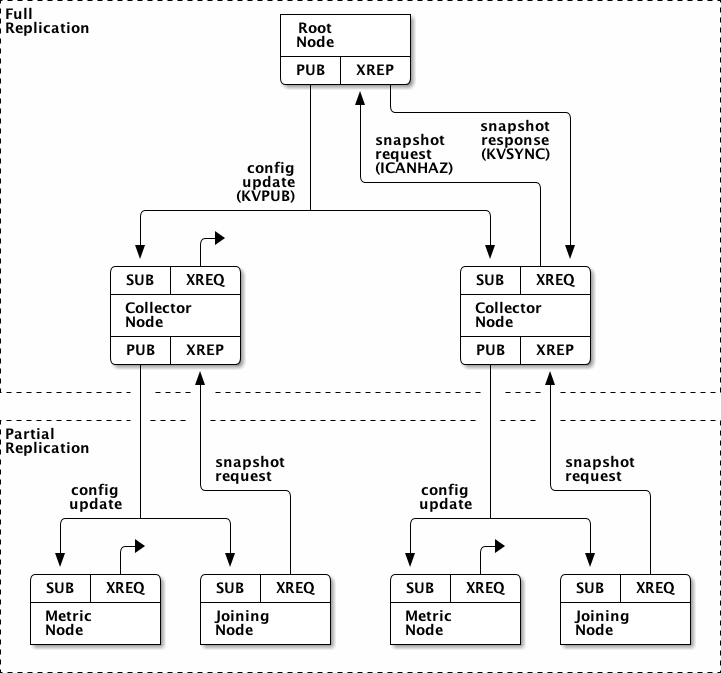
\includegraphics[scale=0.66]{config.png}
    \caption{Configuration Protocol Diagram}
    \label{fig:proto_config_image}
\end{figure}

\subsubsection{Message Definitions}

These messages come from the CHP protocol. Additionally, a \texttt{WTF} error message may be sent by the parent in case
of error. It should be noted, each of the following messages is really the same five-frame format with varying keys and
semantics.

As shown in Figure \ref{fig:proto_config_spec}, the \texttt{ICANHAZ}, \texttt{KVSYNC}, and \texttt{KTHXBAI} messages are
sent across a REQ/REP connection type. \texttt{KVPUB} (as the name would imply) along with the \texttt{HUGZ} heartbeat
message are designed for the PUB/SUB pattern.

\textbf{\texttt{ICANHAZ}} is a configuration snapshot request sent by the child node when it first starts. Multiple
\texttt{ICANHAZ} requests can be sent for the different topics or subtrees needed by the node, and the node will not
begin normal operation until all of the requested values have been received.

\begin{figure}[H]
\vspace{+10pt}
\begin{verbatim}
Frame 0: "ICANHAZ", as 0MQ string
Frame 1: <empty>
Frame 2: <empty>
Frame 3: <empty>
Frame 4: subtree specification, as 0MQ string
\end{verbatim}
\vspace{-20pt}
\caption{\texttt{ICANHAZ} Message Definition}
\label{fig:message_icanhaz}
\end{figure}

\textbf{\texttt{KVSYNC}} is a configuration snapshot response message. For every key-value pair within the requested
subtree, a \texttt{KVSYNC} message is sent to the child node. Note: if no values exist for a requested subtree, a
\texttt{KTHXBAI} message will be the only response received by the child node.

The sequence number in Frame 1 SHOULD be ignored by the recipient since no order guarantees exist for configuration
snapshots requests.

\begin{figure}[H]
\vspace{+10pt}
\begin{verbatim}
Frame 0: key, as 0MQ string
Frame 1: sequence number, 8 bytes in network order
Frame 2: <empty>
Frame 3: <empty>
Frame 4: value, as blob
\end{verbatim}
\vspace{-20pt}
\caption{\texttt{KVSYNC} Message Definition}
\label{fig:message_kvsync}
\end{figure}

\textbf{\texttt{KTHXBAI}} marks the end of a successful snapshot request. Frame 4 MUST contain the highest sequence
number of all the values in the configuration snapshot.

\begin{figure}[H]
\vspace{+10pt}
\begin{verbatim}
Frame 0: "KTHXBAI", as 0MQ string
Frame 1: sequence number, 8 bytes in network order
Frame 2: <empty>
Frame 3: <empty>
Frame 4: subtree specification, as 0MQ string
\end{verbatim}
\vspace{-20pt}
\caption{\texttt{KTHXBAI} Message Definition}
\label{fig:message_kthxbai}
\end{figure}

\textbf{\texttt{KVPUB}} is a configuration update sent from parent to child. The sequence number in Frame 1 must be
monotonically increasing. When a \texttt{KVPUB} is received which has a sequence number lower than a previously received
\texttt{KVPUB}, the node MUST delete its saved configuration values and request a new snapshot.

Frame 2 SHOULD contain the UUID of the node from which the value originated. In \dcamp, this should only be the Root
node's UUID. Frame 3 MAY contain additional properties for the key-value pair, such as an ephemeral time-to-live.

\begin{figure}[H]
\vspace{+10pt}
\begin{verbatim}
Frame 0: key, as 0MQ string
Frame 1: sequence number, 8 bytes in network order
Frame 2: UUID, 16 bytes in network order
Frame 3: properties, JSON-encoded, as 0MQ string
Frame 4: value, as blob
\end{verbatim}
\vspace{-20pt}
\caption{\texttt{KVPUB} Message Definition}
\label{fig:message_kvpub}
\end{figure}

\textbf{\texttt{HUGZ}} is the heartbeat message sent from parent to child when the rate of \texttt{KVPUB} messages being
sent drops below a predetermined threshold. The \texttt{HUGZ} message is critical to maintaining topological consistency
in \dcamp.

\begin{figure}[H]
\vspace{+10pt}
\begin{verbatim}
Frame 0: "HUGZ"
Frame 1: 00000000
Frame 2: <empty>
Frame 3: <empty>
Frame 4: <empty>
\end{verbatim}
\vspace{-20pt}
\caption{\texttt{HUGZ} Message Definition}
\label{fig:message_hugz}
\end{figure}
